\documentclass{article}

% if you need to pass options to natbib, use, e.g.:
    % \PassOptionsToPackage{numbers, compress}{natbib}
% before loading neurips_2020

% ready for submission
% \usepackage{neurips_2020}

% to compile a preprint version, e.g., for submission to arXiv, add add the
% [preprint] option:
    % \usepackage[preprint]{neurips_2020}

% to compile a camera-ready version, add the [final] option, e.g.:
\usepackage[final]{neurips_2020}

% to avoid loading the natbib package, add option nonatbib:
% \usepackage[nonatbib]{neurips_2020}

\usepackage[utf8]{inputenc} % allow utf-8 input
\usepackage[T1]{fontenc}    % use 8-bit T1 fonts
\usepackage{hyperref}       % hyperlinks
\usepackage{url}            % simple URL typesetting
\usepackage{booktabs}       % professional-quality tables
\usepackage{amsfonts}       % blackboard math symbols
\usepackage{nicefrac}       % compact symbols for 1/2, etc.
\usepackage{microtype}      % microtypography
\usepackage{graphicx}
\graphicspath{ {../plots} }

\title{Multi-Class Sentiment Analysis on Amazon Fine Food Reviews}

% The \author macro works with any number of authors. There are two commands
% used to separate the names and addresses of multiple authors: \And and \AND.
%
% Using \And between authors leaves it to LaTeX to determine where to break the
% lines. Using \AND forces a line break at that point. So, if LaTeX puts 3 of 4
% authors names on the first line, and the last on the second line, try using
% \AND instead of \And before the third author name.

\author{%
  Nikolaos Gounakis\\
  Department of Computer Science\\
  University of Crete\\
  Voutes University Campus, 700 13 Heraklion, Crete, Greece\\
  \texttt{nicolaig@csd.uoc.gr} \\
  % examples of more authors
  % \And
  % Coauthor \\
  % Affiliation \\
  % Address \\
  % \texttt{email} \\
  % \AND
  % Coauthor \\
  % Affiliation \\
  % Address \\
  % \texttt{email} \\
  % \And
  % Coauthor \\
  % Affiliation \\
  % Address \\
  % \texttt{email} \\
  % \And
  % Coauthor \\
  % Affiliation \\
  % Address \\
  % \texttt{email} \\
}

\begin{document}

\maketitle

\begin{abstract}
In Web applications it is useful to understand various concepts of text. 
One of them is the ability to understand if a piece of text provides a negative,
a positive or a neutral meaning. That can result to a new way of producing analytics 
for users when analyzing reviews or social media posts. In this study we compare
2 techniques as \cite{studyPaper} TF-IDF \cite{tfidf} and Doc2Vec \cite{doc2vec} 
for feature extraction of text data and evaluate them comparing also 5 machine learning algorithms. 
In order to do that we use the Amazon Fine Food reviews dataset \cite{amzfood}.
\end{abstract}

\section{Introduction}
Text classification in a really challenging process. Machine learning techniques 
such as feature extraction enables us to map high dimensional data to a smaller 
number of variables. In our case text is the high dimensional input and using 
TF-IDF and doc2vec we will extract variables that represent this text in a 
lower dimension.

The Growth of modern web apps, such as Tweeter, Facebook and the million 
posts of users have brought in the surface the need of these big companies to 
analyze and gain information of these posts or reviews in our case. That will
enable the companies to have better analytics (analyze feedback) and also 
spotting users that create unwanted content in the platform. 

\section{Dataset}
This dataset consists of reviews of fine foods from Amazon. 
The data span a period of more than 10 years, including all 568,454 reviews 
up to October 2012. Reviews include product and user information, ratings, and a plain text review. 
It also includes reviews from all other Amazon categories.
\url{https://www.kaggle.com/snap/amazon-fine-food-reviews}

The main columns of the dataset that we use were the:
\begin{itemize}
  \item Score: ranges from 1 to 5 indicating good or bad review
  \item Summary: a short description of the review
  \item Text: the actual review
\end{itemize}

From those 3 will proceeded with the \textbf{Score} and the \textbf{Text}.

\begin{figure}
  \begin{subfigure}[b]{0.4\linewidth}
  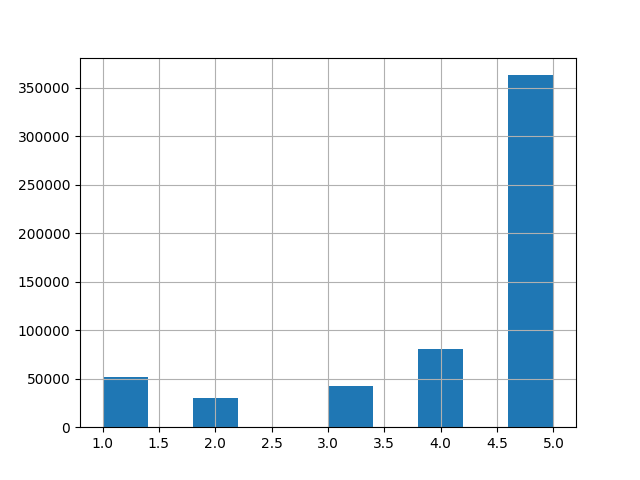
\includegraphics[width=\linewidth]{Score5.png}
  \caption{Score value distribution}
  \label{fig:Score5}
\end{subfigure}

\begin{subfigure}[b]{0.4\linewidth}
  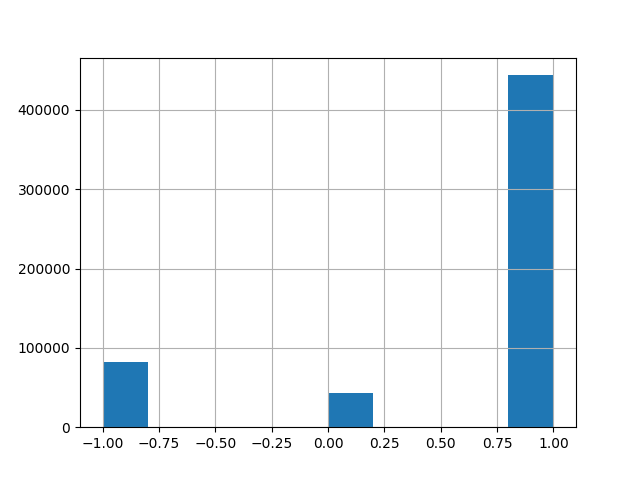
\includegraphics[width=\linewidth]{Score3.png}
  \caption{Score value distribution after reduction}
  \label{fig:Score3}
\end{subfigure}
\end{figure}

\section{Methodology}

\section{Experiments}

\begin{table}[h]
  \begin{tabular}{lllllll}
  \hline
  Feature Extraction Method & \multicolumn{3}{l}{TF-IDF}                          & \multicolumn{3}{l}{Doc2Vec}                         \\ \hline
                            & Accuracy        & F1              & AUC             & Accuracy        & F1              & AUC             \\ \hline
  KNN (n=5)                 & 47.990          & 46.228          & 65.965          & 39.580          & 39.367          & 56.897          \\
  SVM-rbf                   & \textbf{64.910} & \textbf{64.883} & \textbf{82.694} & \textbf{44.139} & \textbf{43.741} & \textbf{62.465} \\
  Logistic Regression       & 63.080          & 62.941          & 80.915          & 37.909          & 37.087          & 54.663          \\
  RF                        & 40.519          & 40.473          & 58.931          & 40.519          & 40.473          & 58.931          \\
  NB                        & 36.980          & 31.211          & 55.265          & 36.980          & 31.211          & 55.265          \\ \hline
  \end{tabular}
  \caption{Multi-Class Classification scores with weighted AUC}
\end{table}

\begin{table}[h]
  \begin{tabular}{lllllll}
  \hline
  Feature Extraction Method & \multicolumn{3}{l}{TF-IDF}                          & \multicolumn{3}{l}{Doc2Vec}                         \\ \hline
                            & Accuracy        & F1              & AUC             & Accuracy        & F1              & AUC             \\ \hline
  KNN (n=5)                 & 71.120          & 71.888          & 71.132          & 58.710          & 63.232          & 58.425          \\
  SVM-rbf                   & \textbf{83.670} & \textbf{83.569} & \textbf{83.668} & \textbf{63.540} & \textbf{66.232} & \textbf{63.374} \\
  Logistic Regression       & 82.780          & 82.684          & 82.778          & 57.980          & 63.065          & 57.657          \\
  RF                        & 81.580          & 81.435          & 81.577          & 59.949          & 60.927          & 59.924          \\
  NB                        & 79.260          & 79.566          & 79.267          & 54.190          & 63.736          & 53.533          \\ \hline
  \end{tabular}
  \caption{Binary Classification scores}
\end{table}
  
\section{Colnclusions}


\bibliographystyle{plain}
\bibliography{bib/report}


\end{document}